% Options for packages loaded elsewhere
\PassOptionsToPackage{unicode}{hyperref}
\PassOptionsToPackage{hyphens}{url}
%
\documentclass[
]{article}
\usepackage{amsmath,amssymb}
\usepackage{iftex}
\ifPDFTeX
  \usepackage[T1]{fontenc}
  \usepackage[utf8]{inputenc}
  \usepackage{textcomp} % provide euro and other symbols
\else % if luatex or xetex
  \usepackage{unicode-math} % this also loads fontspec
  \defaultfontfeatures{Scale=MatchLowercase}
  \defaultfontfeatures[\rmfamily]{Ligatures=TeX,Scale=1}
\fi
\usepackage{lmodern}
\ifPDFTeX\else
  % xetex/luatex font selection
\fi
% Use upquote if available, for straight quotes in verbatim environments
\IfFileExists{upquote.sty}{\usepackage{upquote}}{}
\IfFileExists{microtype.sty}{% use microtype if available
  \usepackage[]{microtype}
  \UseMicrotypeSet[protrusion]{basicmath} % disable protrusion for tt fonts
}{}
\makeatletter
\@ifundefined{KOMAClassName}{% if non-KOMA class
  \IfFileExists{parskip.sty}{%
    \usepackage{parskip}
  }{% else
    \setlength{\parindent}{0pt}
    \setlength{\parskip}{6pt plus 2pt minus 1pt}}
}{% if KOMA class
  \KOMAoptions{parskip=half}}
\makeatother
\usepackage{xcolor}
\usepackage[margin=1in]{geometry}
\usepackage{graphicx}
\makeatletter
\def\maxwidth{\ifdim\Gin@nat@width>\linewidth\linewidth\else\Gin@nat@width\fi}
\def\maxheight{\ifdim\Gin@nat@height>\textheight\textheight\else\Gin@nat@height\fi}
\makeatother
% Scale images if necessary, so that they will not overflow the page
% margins by default, and it is still possible to overwrite the defaults
% using explicit options in \includegraphics[width, height, ...]{}
\setkeys{Gin}{width=\maxwidth,height=\maxheight,keepaspectratio}
% Set default figure placement to htbp
\makeatletter
\def\fps@figure{htbp}
\makeatother
\setlength{\emergencystretch}{3em} % prevent overfull lines
\providecommand{\tightlist}{%
  \setlength{\itemsep}{0pt}\setlength{\parskip}{0pt}}
\setcounter{secnumdepth}{-\maxdimen} % remove section numbering
\ifLuaTeX
  \usepackage{selnolig}  % disable illegal ligatures
\fi
\usepackage{bookmark}
\IfFileExists{xurl.sty}{\usepackage{xurl}}{} % add URL line breaks if available
\urlstyle{same}
\hypersetup{
  pdftitle={AFP},
  pdfauthor={Anoosha Imran},
  hidelinks,
  pdfcreator={LaTeX via pandoc}}

\title{AFP}
\author{Anoosha Imran}
\date{2025-02-23}

\begin{document}
\maketitle

\section{Final Proposal}\label{final-proposal}

I ended up changing my initial project. I wanted to do a project which
relates to my area of study. For my final project In will be looking at
the School Absenteeism in the United States.

My first three sketches are just an attempt at me understanding what I
can do with the data. I wanted to map the count of absenteeism against
the years and the States to see what kind of visualisation I can come up
with.

\section{Sketch 1}\label{sketch-1}

\begin{figure}
\centering
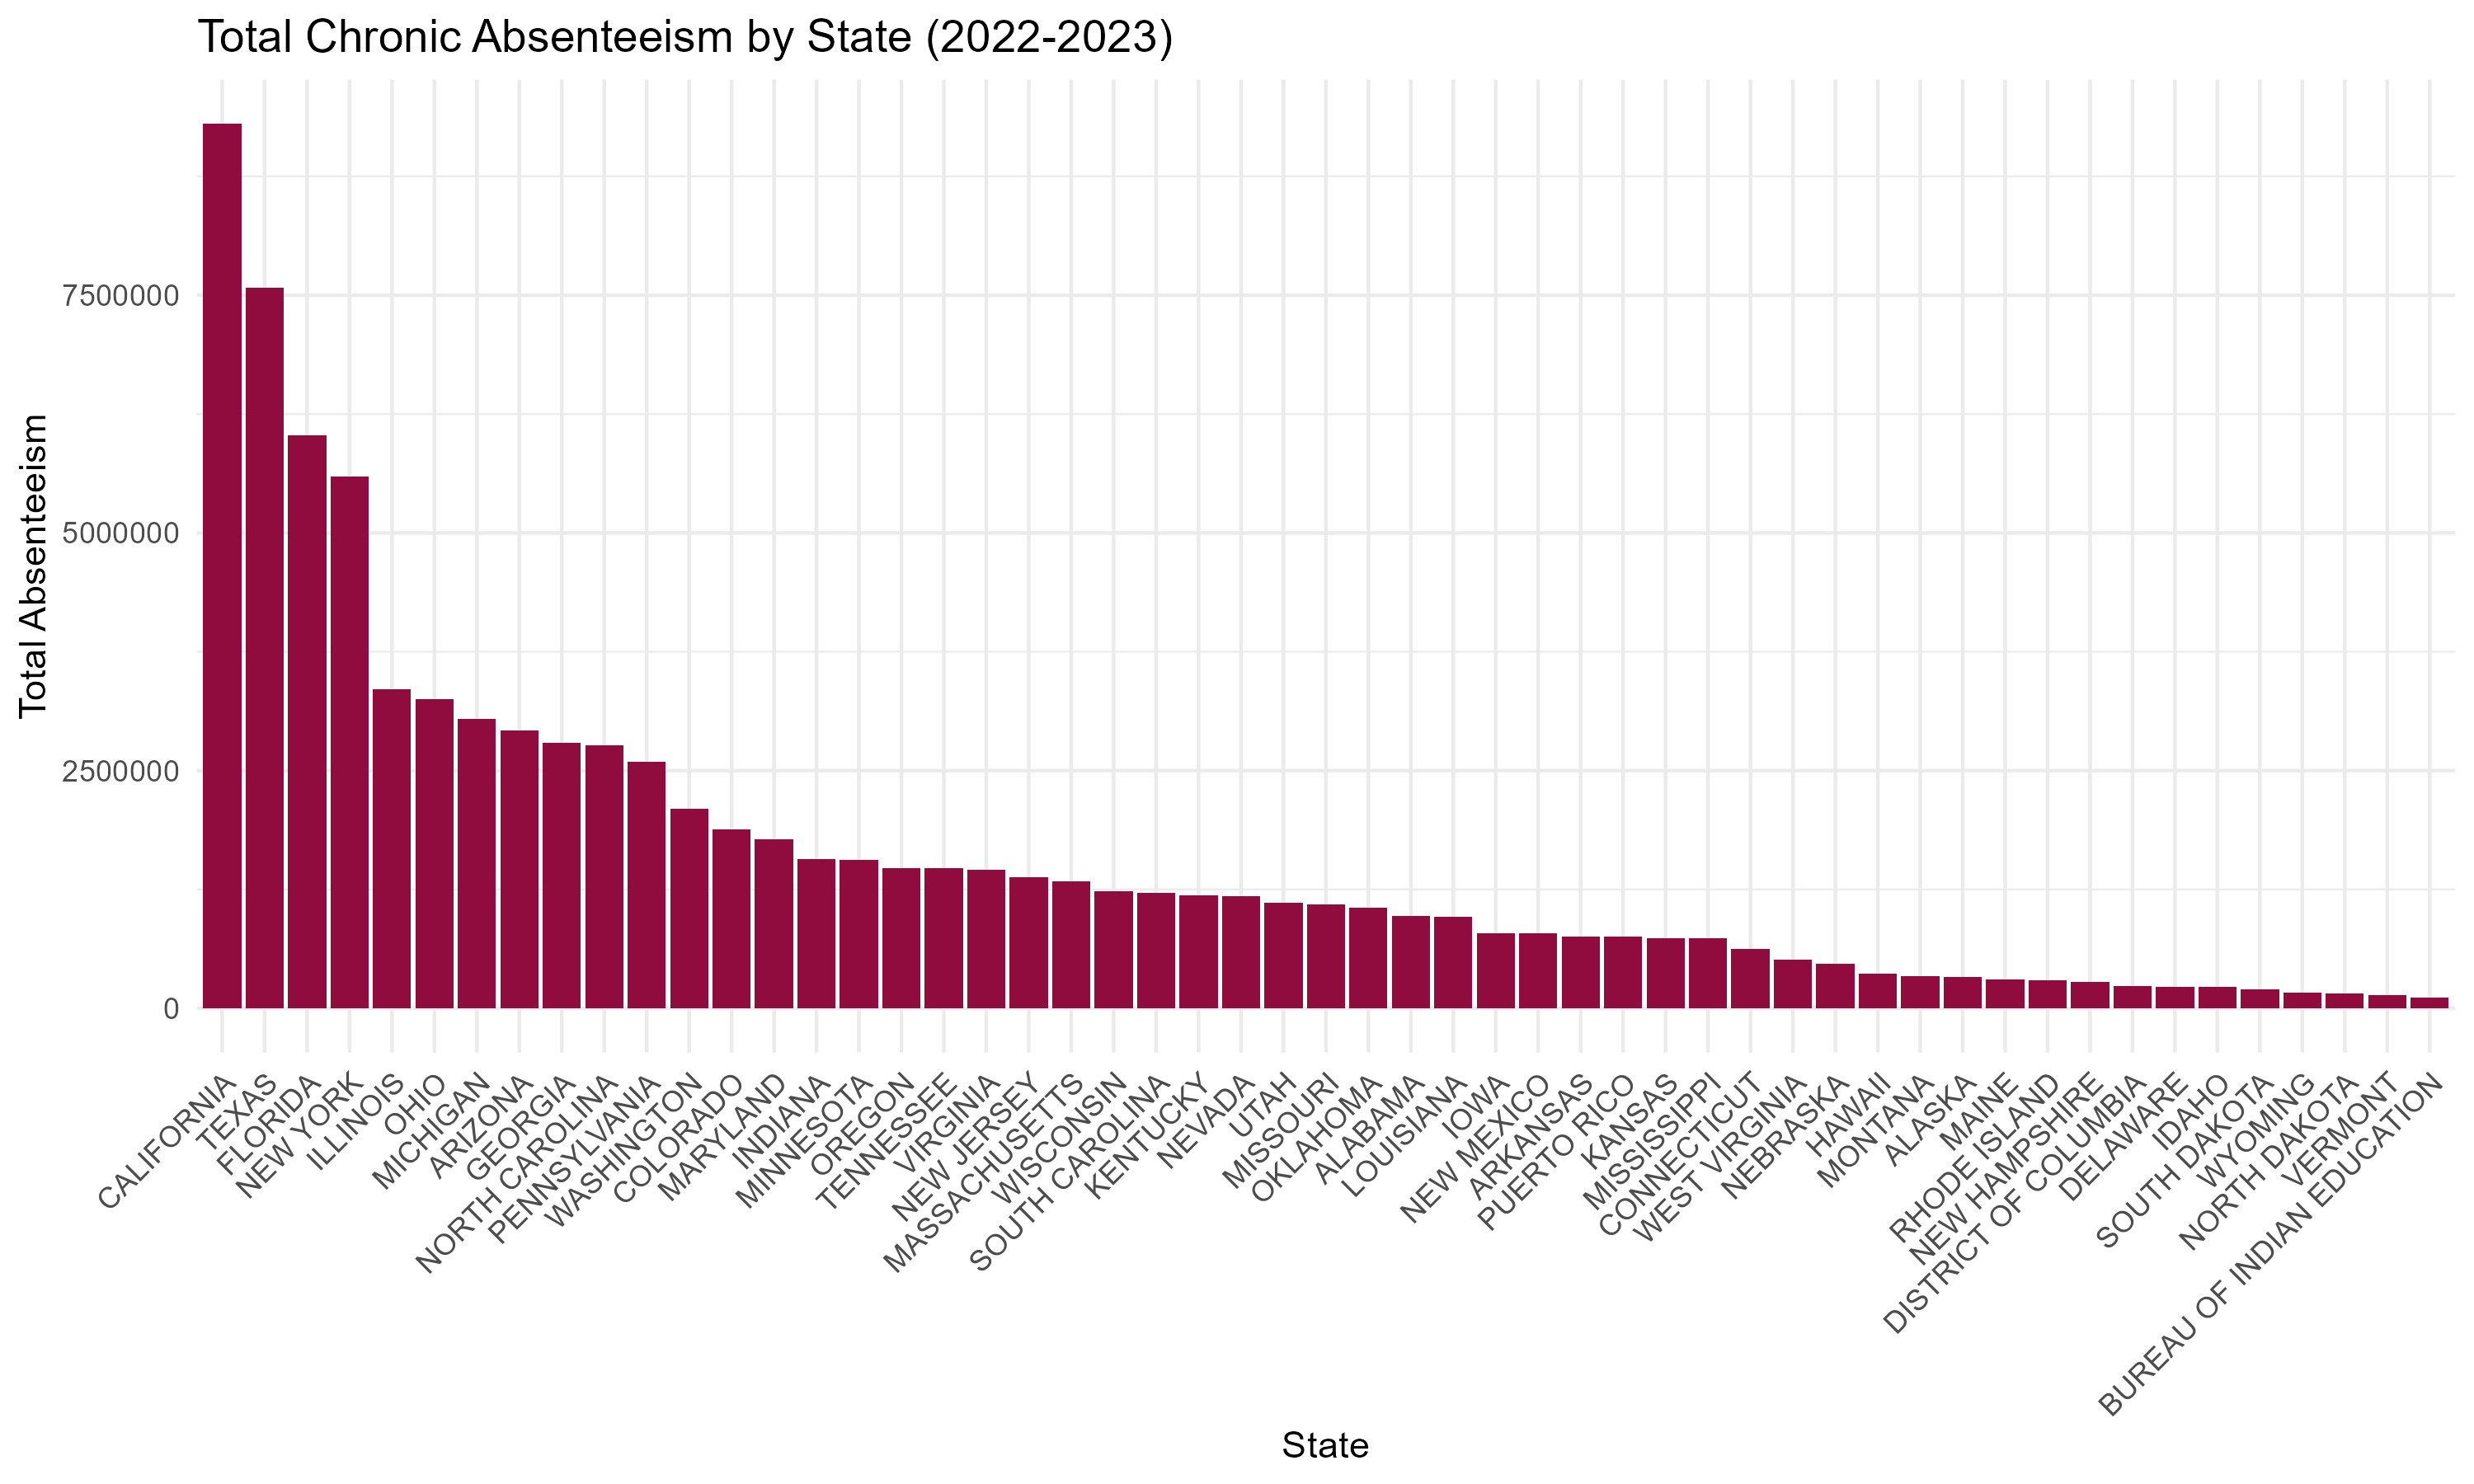
\includegraphics{Sketch 1.png}
\caption{My Plot}
\end{figure}

\section{Sketch 2}\label{sketch-2}

\begin{figure}
\centering
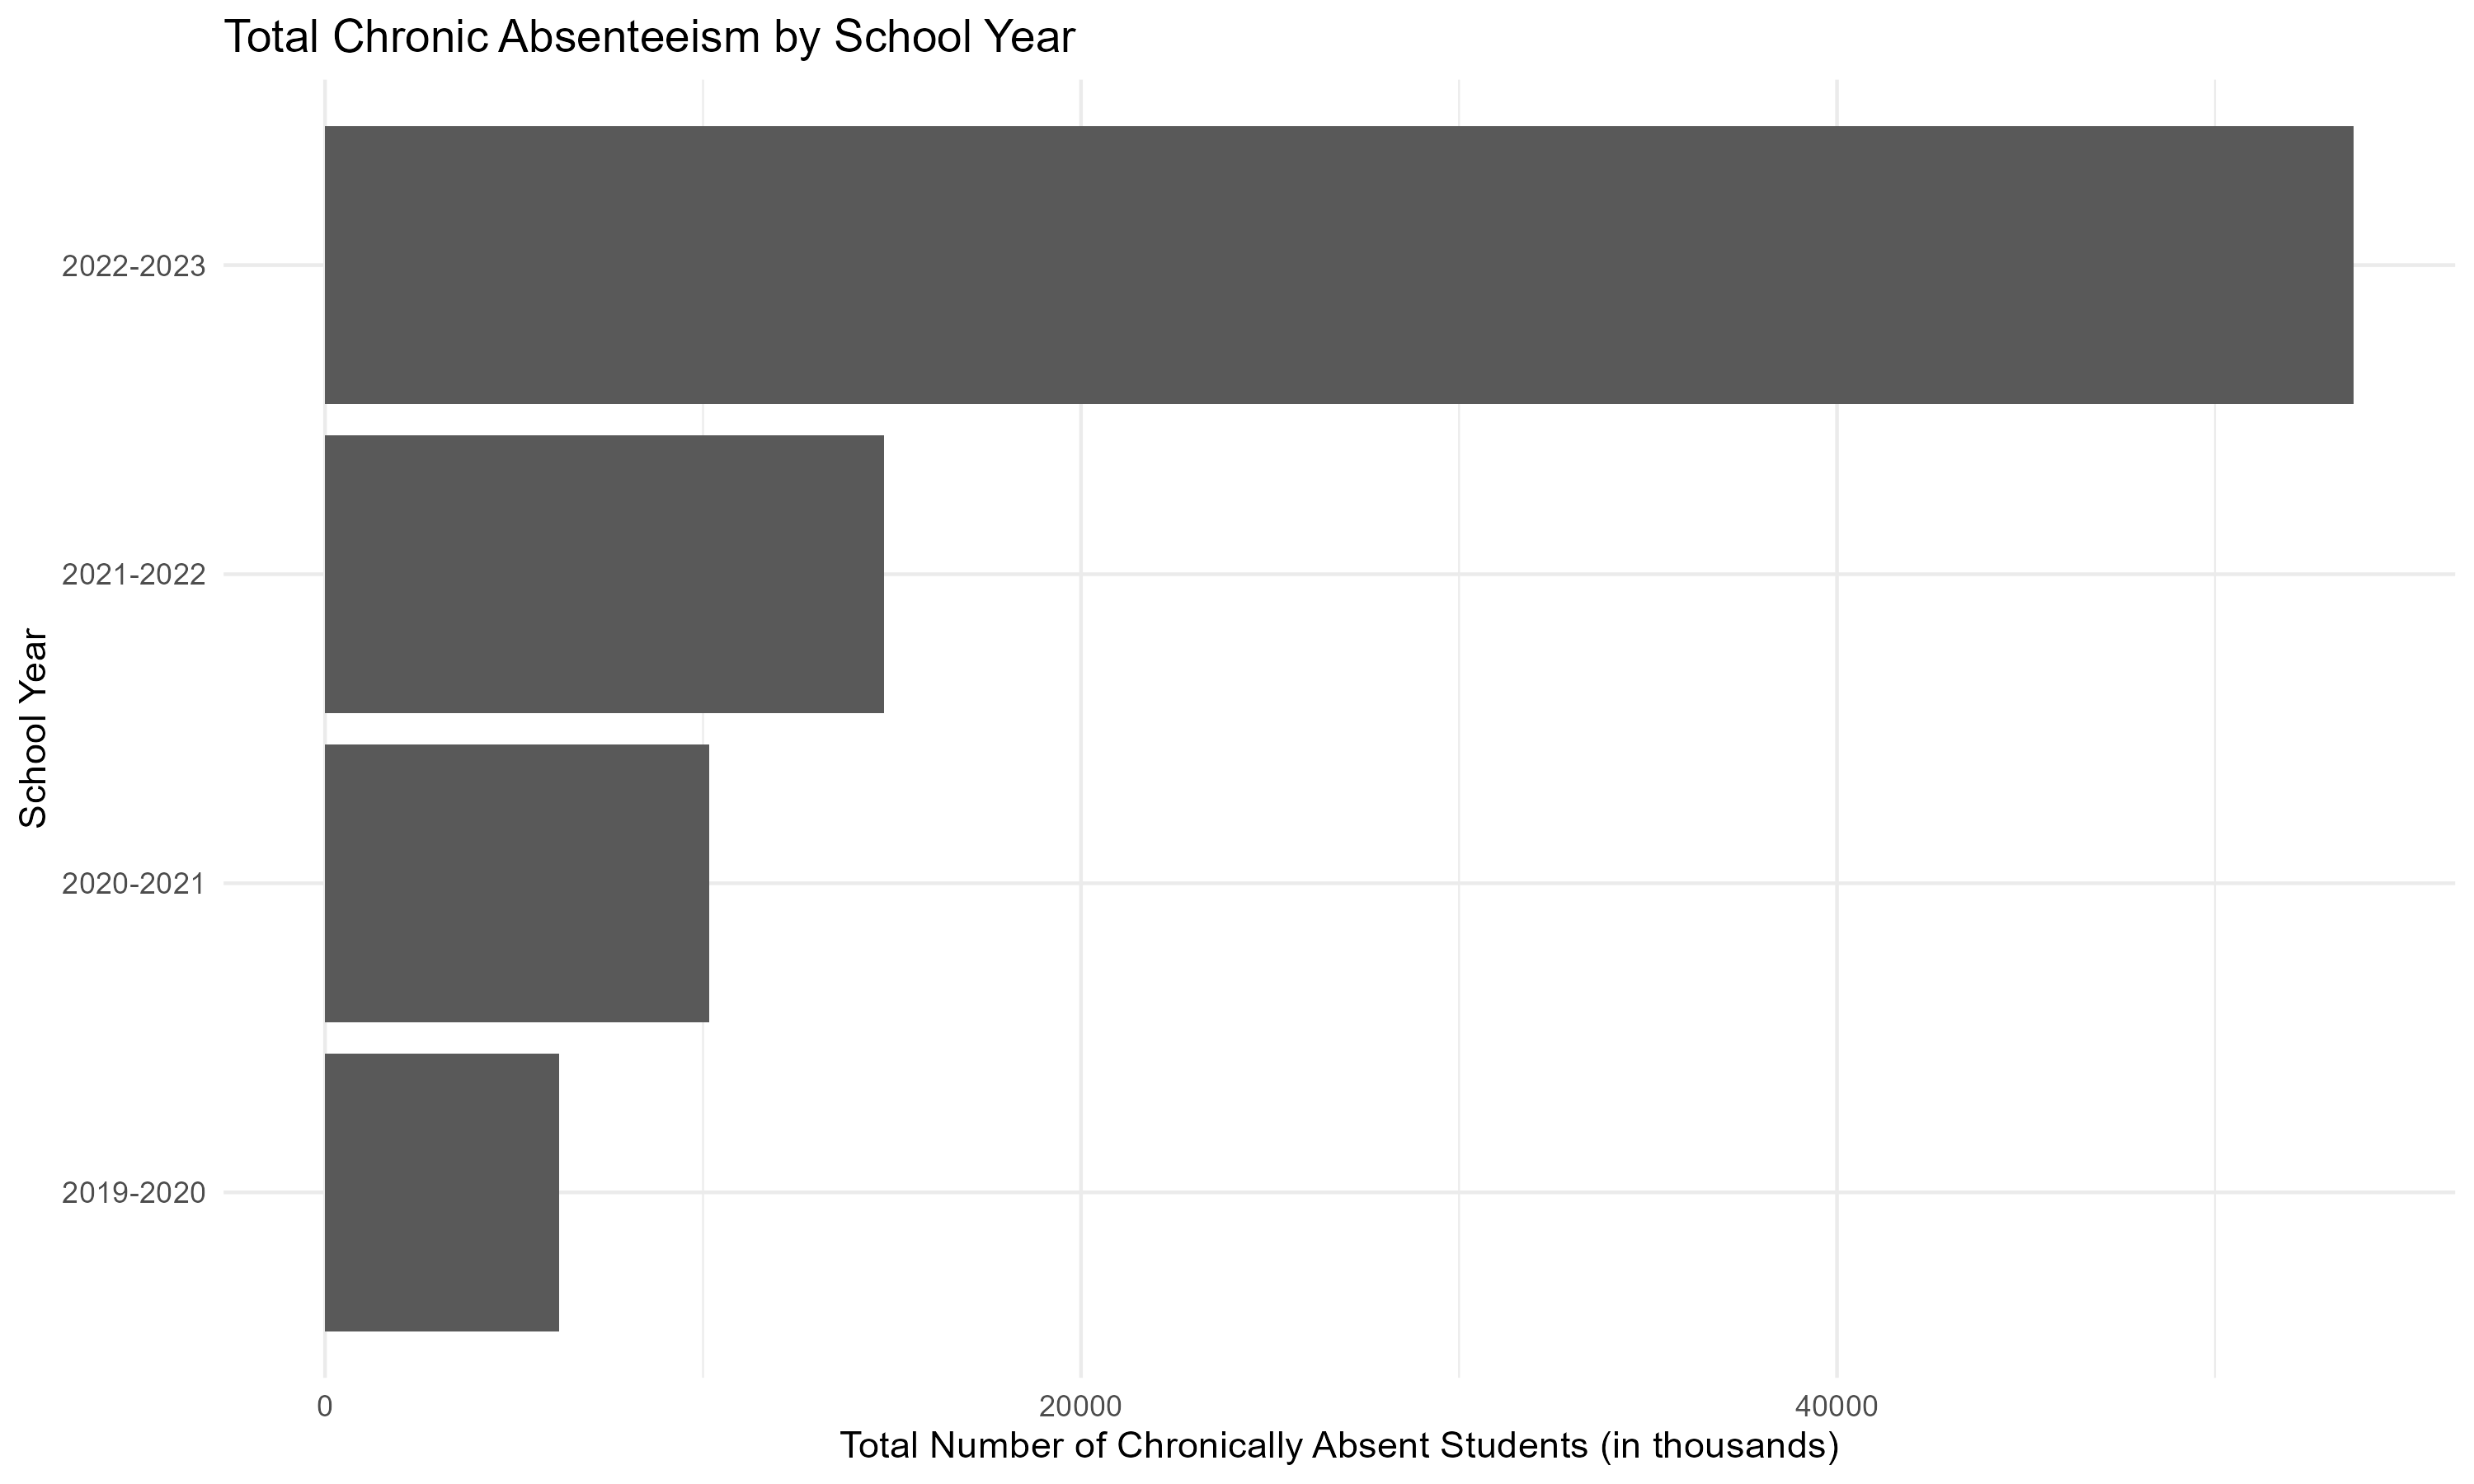
\includegraphics{Sketch 2.png}
\caption{My Plot}
\end{figure}

\section{Sketch 3}\label{sketch-3}

\begin{figure}
\centering
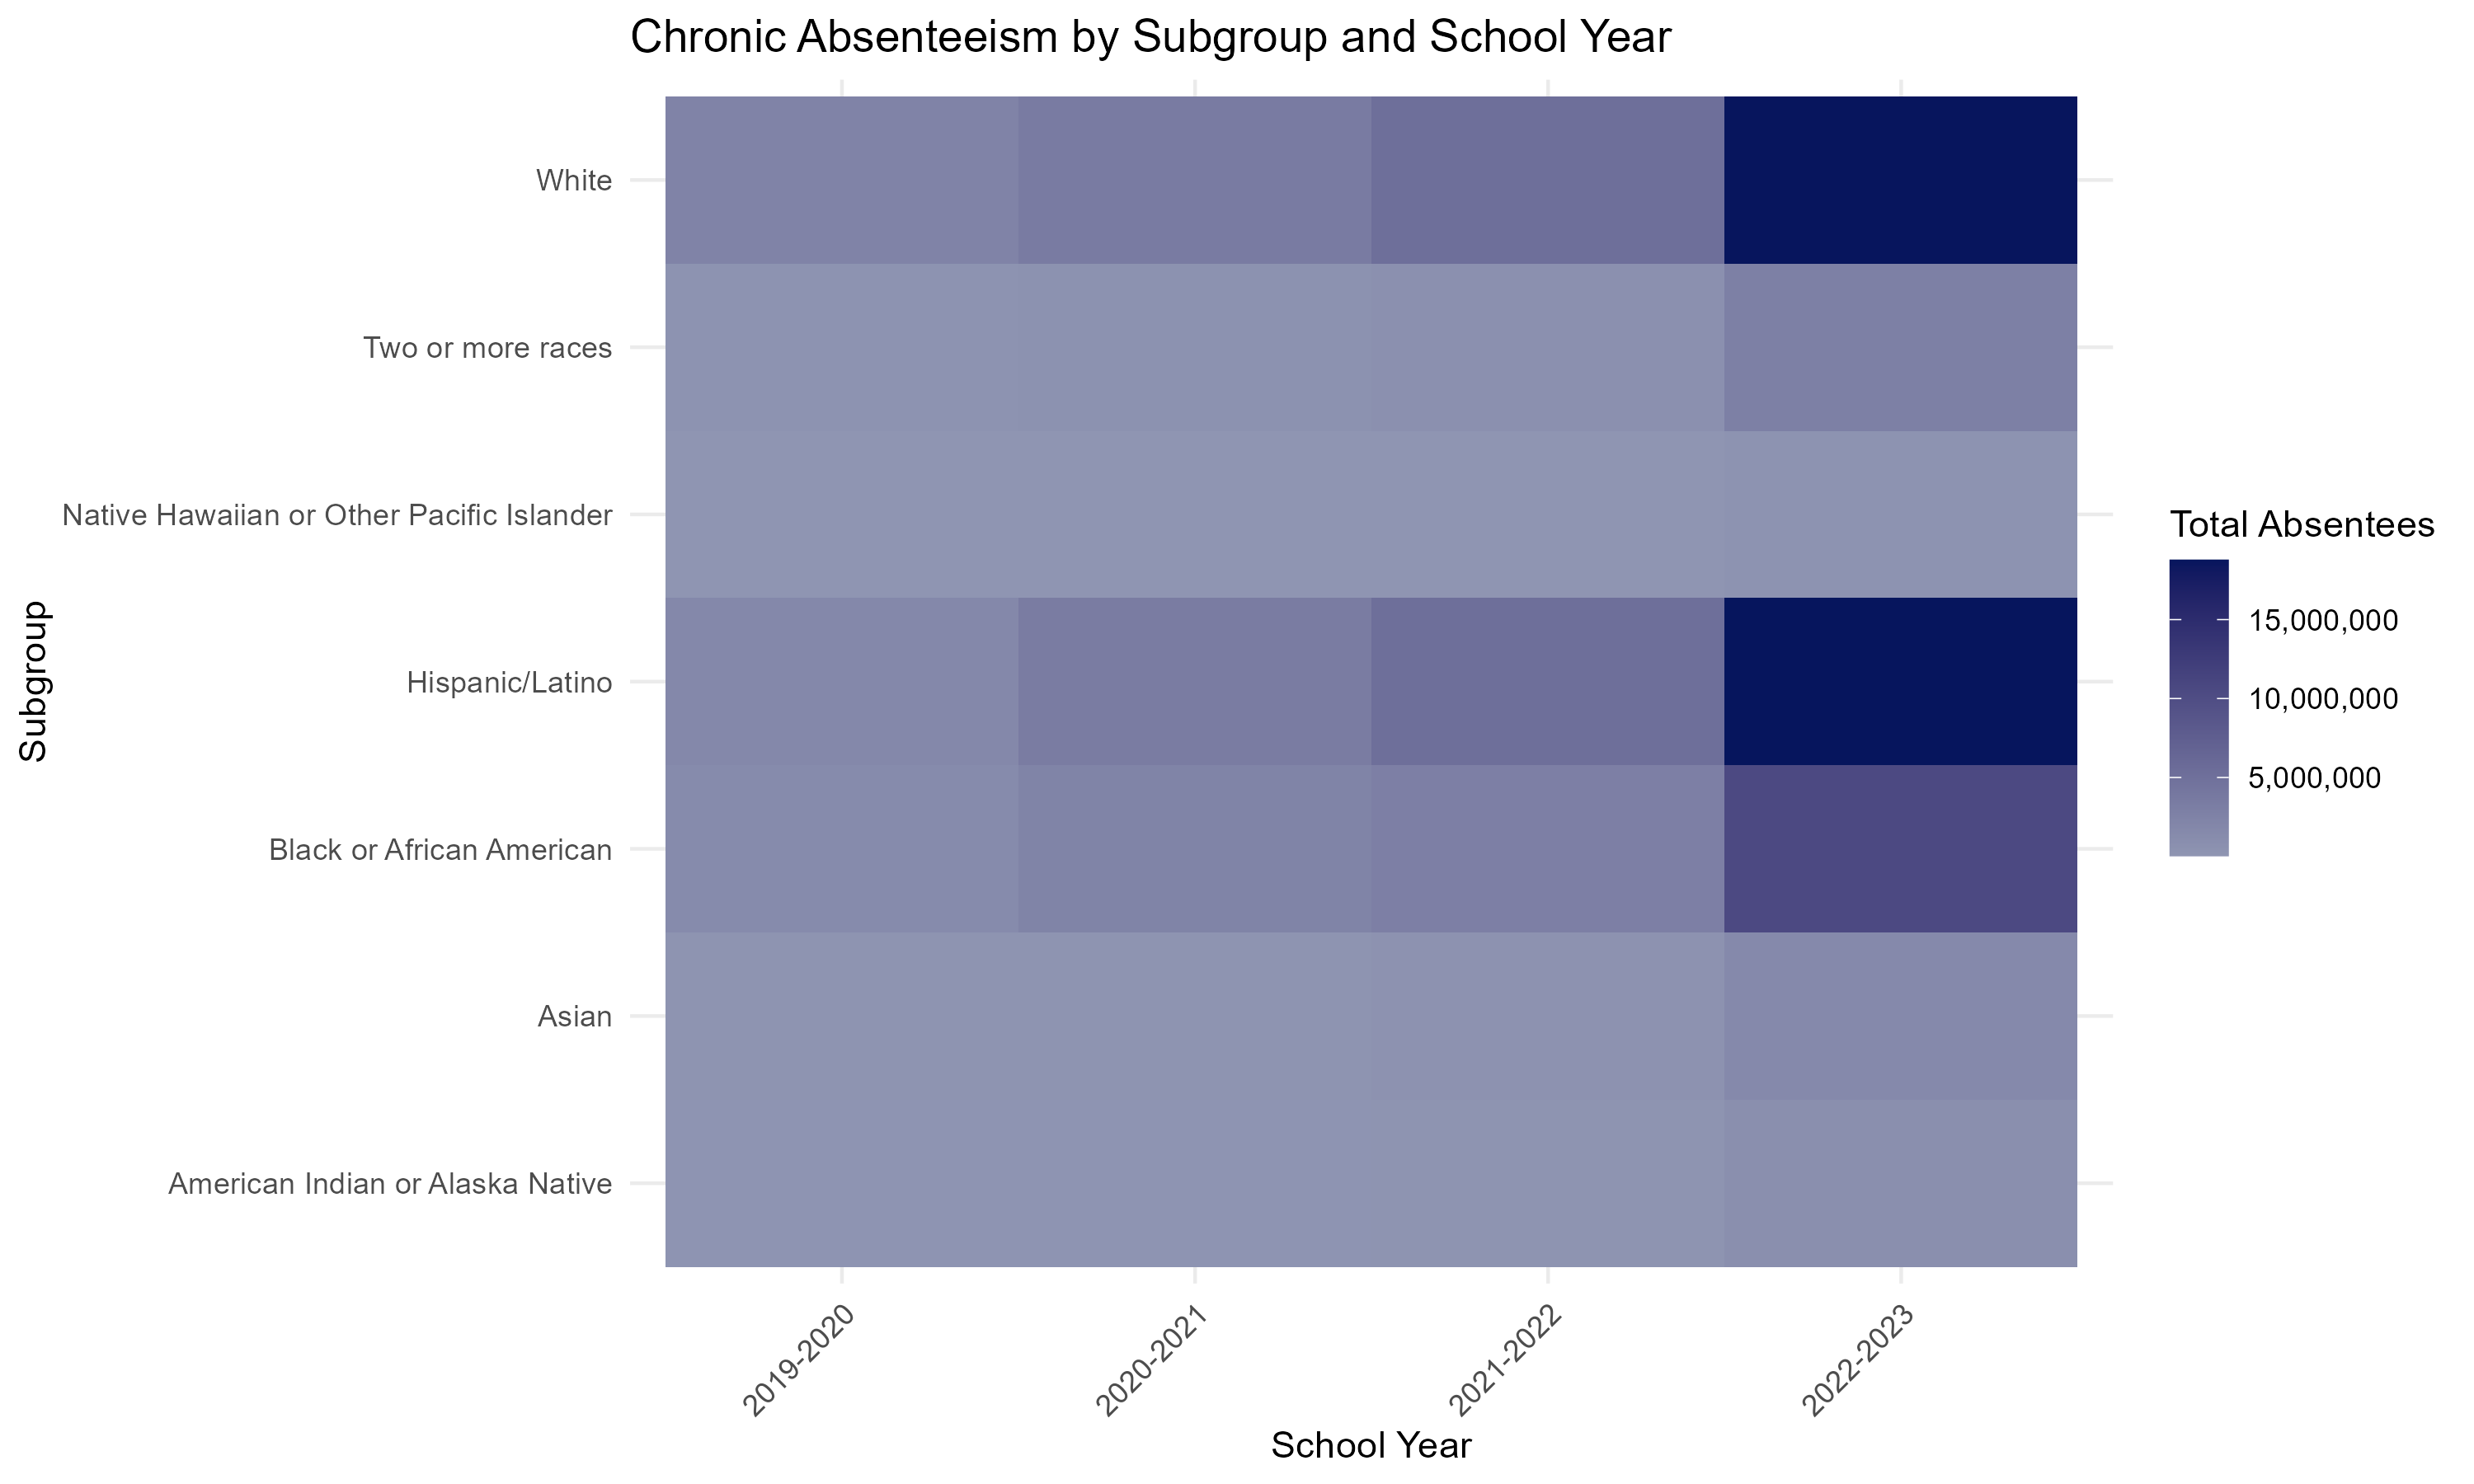
\includegraphics{Sketch 3.png}
\caption{My Plot}
\end{figure}

The initial dataset provides a detailed breakdown of chronic absenteeism
across US schools, categorized by state, subgroup (e.g., race/ethnicity,
gender), and other demographic characteristics. To gain a high-level
understanding of this complex data, I created a map. This map visualizes
the total chronic absenteeism rates for each state, using a color
gradient to represent the magnitude of the problem. By hovering over
each state, users can see a breakdown of absenteeism by gender,
providing insights into how this issue affects different student
populations across the country. This visualization allows for quick
identification of states with the highest absenteeism rates and
highlights disparities within those states.

!{[}My Plot{]} (Final\_plot.html)

\href{file:///E:/RStudio/ProjectProposal/Final_plot.html}{\includegraphics{Final_plot.html}}

As I move towards my final project, my plan is to enhance my final
visualisation and create a dashboard with updated data to show the trend
of absenteeism across the United States and attempt to plot it agaist
the growing impact of Climate Change so see whether it has an impact or
not.

\end{document}
